In this chapter we will make a comparison between the simulation using the full set of CELMA equations (\textbf{C}ELMA-\textbf{F}ull, or simply CF), with the simulations using the Boussinesq approximation (\textbf{C}ELMA-\textbf{B}oussinesq, or simply CB).
We will see that the missing $n$ in the voriticity equation causes a difference in the parallel electron and ion flux, and that the energy will drift with time.

\section{Steady state profiles}
%
\begin{figure}[h]
    \centering
    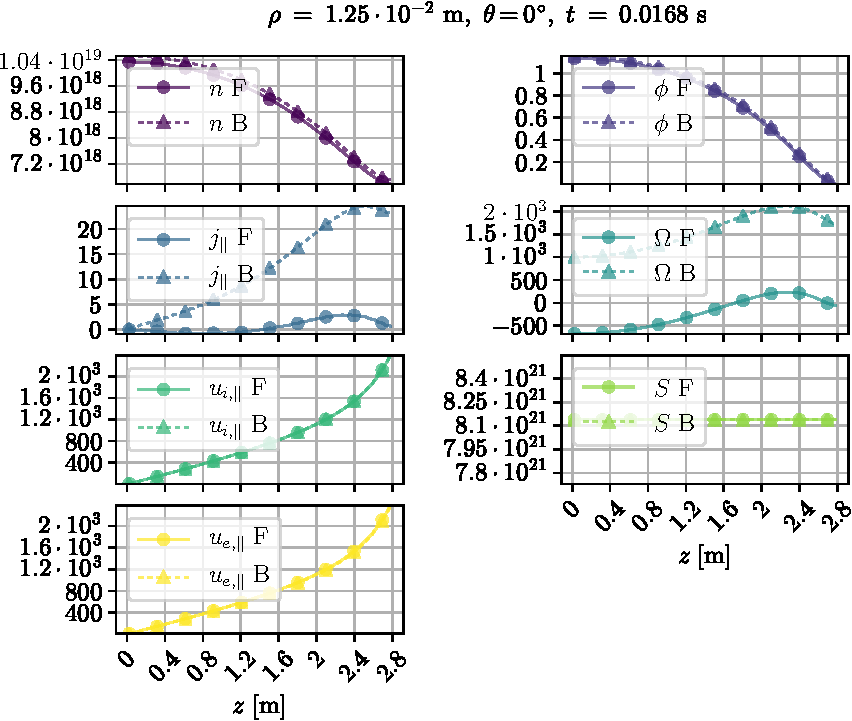
\includegraphics{fig/results/compareBouss/1DProfRad001B}
    \caption{Radial steady state profiles with and without the Boussinesq approximation for $B_0=0.1\T$.
        Dots denotes the full simulation (but does not indicate the location of a grid point).
        Triangles denotes the simulation with the Boussinesq approximation (but does not indicate the location of a grid point).
        The units are the same as those used in \cref{fig:radProfs}.
    }
    \label{fig:compareBoussProfRad}
\end{figure}
%
If we start by comparing the steady state profiles, we can first note that any difference between the CF and the CB model, lays in the vorticity equation.
The biggest difference between \cref{eq:celma_vortD_evolution} and \cref{eq:celma_vort_boussinesq} is how the density factor in the compression of the density times the ion polarization term is treated.
By using the Boussinesq approximation, we assumed that the mentioned $n$ was the same as a flat background $n_0$.
This $n_0$ then got normalized out, meaning that the $n$-dependency in this term disappeared.
As a result, we ended up with a source term in the CB model not present in the CF model, since this term got canceled with the source term from the density equation which we "smuggled" inside the $\d_t^E$ operator in the CF case.
Finally, the $\ve{E}\times\ve{B}$ advection terms are different in the two cases.
These differences affect both the background profiles and the fluctuations.

Hence, it should come as no surprise that the radial vorticity profile has changed.
This is indicated in \cref{fig:compareBoussProfRad}, which shows the difference between the CF and CB simulation for $B=0.1\T$.
As the radial vorticity profiles changes, it will lead to changes in the radial potential profile%
%
\footnote{One could say that it is the potential which determines the vorticity through $\Om = \grad_\perp^2 \phi$, but since we are evolving the vorticity in time we are instead inverting the equation for $\phi$.
In that respect $\Om$ determines $\phi$.}%
%
.
The radial density profile stays roughly the same for the CF and CB case, which will be discussed in further detail below.
For the radial profile of the parallel currents we can observe that the CB case gives slower velocities for the CB case when $\rho \to L_\rho$
This, in turn, makes small changes in the radial parallel current profile, but gives a more shallow approach as $\rho\to L_\rho$.
%
\begin{figure}[h]
    \centering
    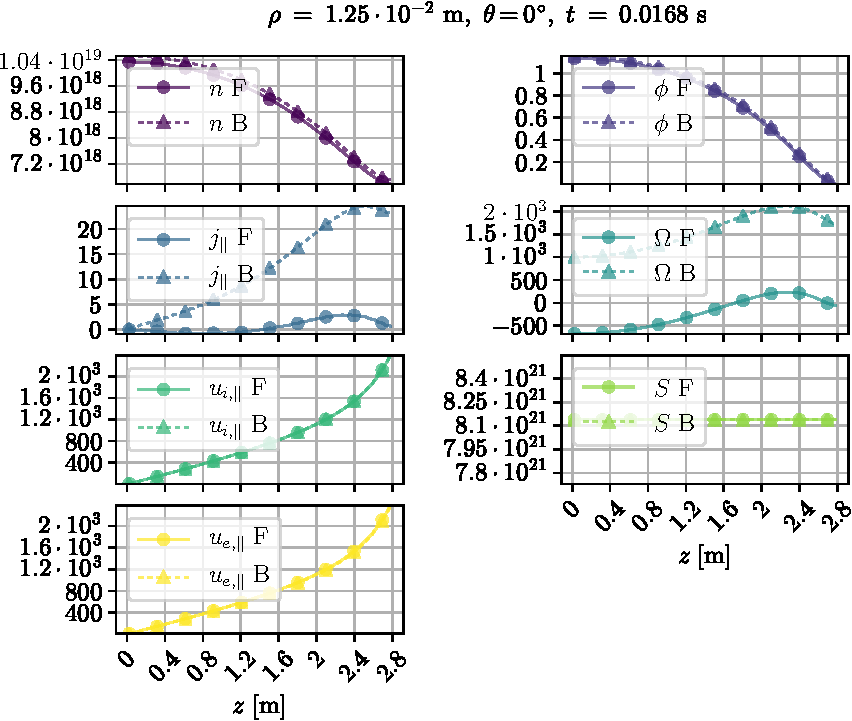
\includegraphics{fig/results/compareBouss/1DProfPar001B}
    \caption{Parallel steady state profiles with and without the Boussinesq approximation for $B_0=0.1\T$.
        Dots denotes the full simulation (but does not indicate the location of a grid point).
        Triangles denotes the simulation with the Boussinesq approximation (but does not indicate the location of a grid point).
        The units are the same as those used in \cref{fig:parProfs}.
    }
    \label{fig:compareBoussProfPar}
\end{figure}
%

On the other hand, the parallel $j_\|$ profile has changed, as seen in \cref{fig:compareBoussProfPar}.
First of all, the see-sawing seen in the non-Boussinesq case seem to have disappeared.
Although the oscillating patterns in the parallel current is still there, they are much less pronounced due to the higher values of $j_\|$.
Secondly the parallel current is around $5$ time larger in magnitude close to the sheath entrance.
This comes from the fact that the balancing terms in the vorticity equation has changed.
In the non-Boussinesq case, the $n$ in $\div(nu_{p,i})$ helped to reduce the terms in the modified vorticity, and thereby the parallel current as $n$ was lower closer to the sheath.
As mentioned above, this $n$ disappears when using the Boussinesq approximation, so it can no longer help to reduce the parallel current.
We can see that this change cannot have its origin in the $\ve{E}\times\ve{B}$ advection terms, as these are not active during the steady state since the $\phi$-field is axisymmetric.
Neither can it origin from the additional source term due to the lack of $n$ dependence.

Due to this, we can observe $\Omega$ has been shifted to a higher value with approximately $1500 \s^{-1}$ in the CB case, and does no longer cross $0$.
In other words, the whole plasma column rotates in the same direction.
Finally, it is worth noting that the system still follows a Boltzmann relation to a high degree, as is the case in the non-Boussinesq case.
This can also explain why the density profile in the CB case is almost the same as in the CF case in the radial direction, as the Boltzmann relation approximately holds for each magnetic field line.
%

\section{The linear state}
%
The change in the vorticity equation has a profound effect on the linear phase.
In the CF case, identifying the linear phase based on the definition given in \cref{chap:linear} was fairly straight forward.
In the CB case the time trace of the Fourier modes are a bit more complicated.
An example of this is shown in \cref{fig:FFTCompB}.
%
\begin{figure}[htbp]
    \centering
    \begin{subfigure}[h]{0.45\textwidth}
        \hspace*{-1cm}
        \centering
        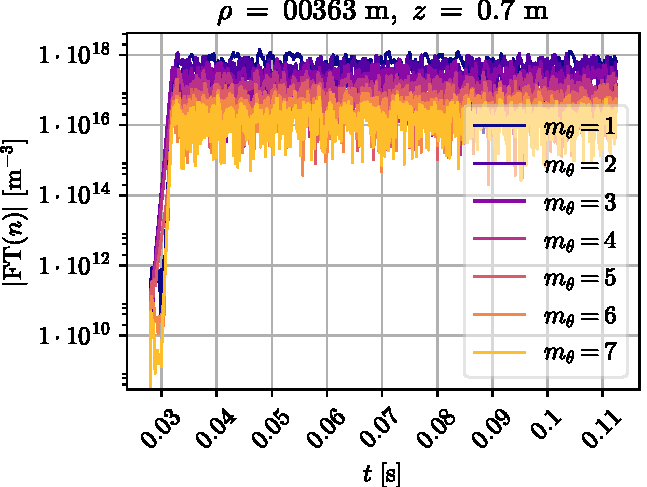
\includegraphics{fig/results/compareBouss/FFT006}
        \caption{Without the Boussinesq approximation.}
        \label{fig:FFTWOB}
    \end{subfigure}%
    \hfill
    \begin{subfigure}[h]{0.45\textwidth}
        \hspace*{-1cm}
        \centering
        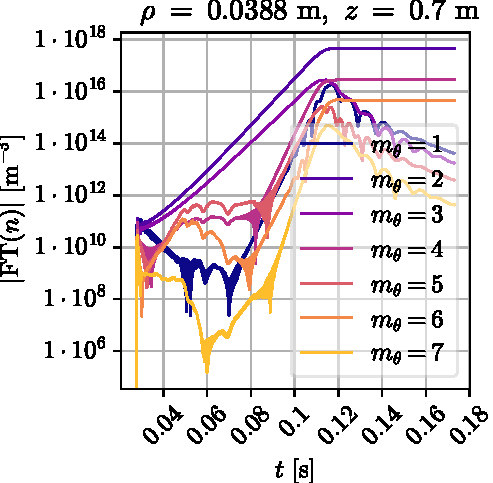
\includegraphics{fig/results/compareBouss/FFT006B}
        \caption{With the Boussinesq approximation.}
        \label{fig:FFTWB}
    \end{subfigure}
    \caption{The time trace of the absolute value of the Fourier modes for $B_0=0.06\T$ for the non-Boussinesq and the Boussinesq case at the position of maximum linear gradient.
    }
    \label{fig:FFTCompB}
\end{figure}
%
In the CF case (\cref{fig:FFTWOB}), the perturbations shows a clear exponential growth.
The intermediate phase between the linear phase and the saturated phase is relatively short.
The CB case (\cref{fig:FFTWB}) has a very short exponential growth after the initial perturbations have died out.
This is followed by a rather long phase where the modes at some times are growing, whilst at others decaying.
The final state for $B_0=0.06\T$ seems to be indeterminate.
Some modes are decaying, whereas the modes with the largest amplitudes are neither growing nor decaying.

Although challenging, we can still try to find the dispersion from the definition of the linear phase given in \cref{chap:linear}.
The result is given in \cref{fig:GRBM,fig:GRBB}.
%
\begin{figure}[htbp]
    \centering
    \begin{subfigure}[h]{0.45\textwidth}
        \centering
        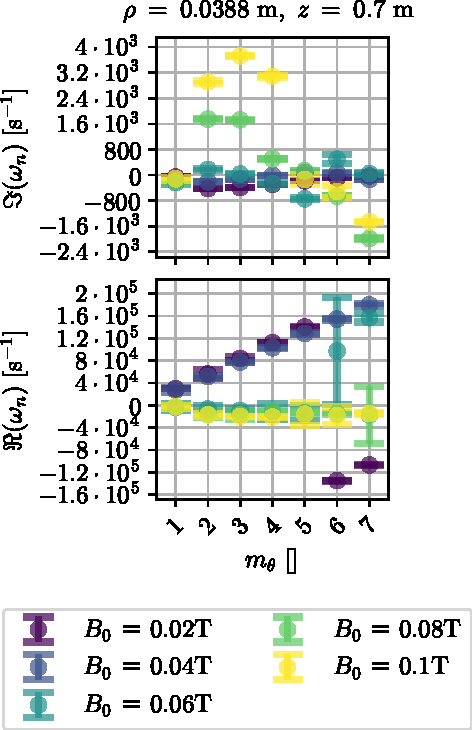
\includegraphics{fig/results/compareBouss/growthRatesB0ModeNr}
        \caption{The growth rates and angular frequencies as a function of $B_0$.}
        \label{fig:GRBB}
    \end{subfigure}
    \hfill
    \begin{subfigure}[h]{0.45\textwidth}
        \centering
        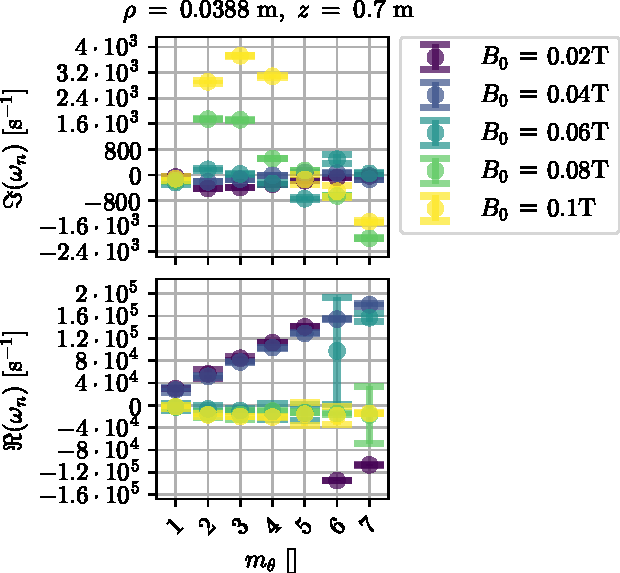
\includegraphics{fig/results/compareBouss/growthRatesB0Bous}
        \caption{The growth rates and angular frequencies as a function of the mode number.}
        \label{fig:GRBM}
    \end{subfigure}%
    \caption{The growth rates and angular frequencies in the CB case.}
    \label{fig:GRB}
\end{figure}
%
From \cref{fig:GRBM}, we can see that the growth rates of the modes are still increasing with increasing $B$-field.
However, the maximum growth is observed in one mode number less than compared with the CF case.
There is also a steeper decrease in the growth rates for higher mode numbers in the CR case.
We observe that the maximum growth rates for the individual $B$-fields is less than half of what it is in the CF case.
One should also emphasize that in the CB case, only $B_0 \geq 0.08\T$ reaches the saturated%
\footnote{As will be shown in \cref{sec:turbB}, the turbulence in the Boussinesq approximation does not really saturate in terms of energy.
    We will still refer to this state as "saturated" in the CB case to distinguish it from the intermediate turbulent phase preceeding the linear state.
} %
%
turbulent state, compared with $B_0 \geq 0.06\T$ in the CF case.

The real part of the dispersion relation is also quite different from the CF case.
As in the CF case, the decaying perturbations for $B_0 \geq 0.02\T$ in the CB case is rotating in the ion diamagnetic direction, but with a rate almost $10$ times higher than compared with the CF case.
This trend ceases for mode $6$ and $7$, where the CB modes suddenly rotates strongly in the electron diamagnetic direction.
A bigger difference is it that in the CB case, also $B_0 = 0.04\T$ rotates in the ion diamagnetic direction, and also exceeds the rotation velocity of the $B_0 = 0.02\T$ case.
Only $B_0 \geq 0.06\T$ shows rotation in the electron diamagnetic direction.
For these magnetic field strengths the rotation increases with increasing magnetic field strength (with exception of the highest modes in $B_0 = 0.06\T$, which rotates in the ion diamagnetic direction).
This is also what was found in the CF case.
% FIXME: Explain why

\section{The turbulence phase}
\label{sec:turbB}
%
There is also a large difference between the Boussinesq and the non-Boussinesq case in the turbulent state.
When investigating the energy in \cref{fig:energies008B} we notice three things.
%
\begin{figure}[htb]
    \centering
    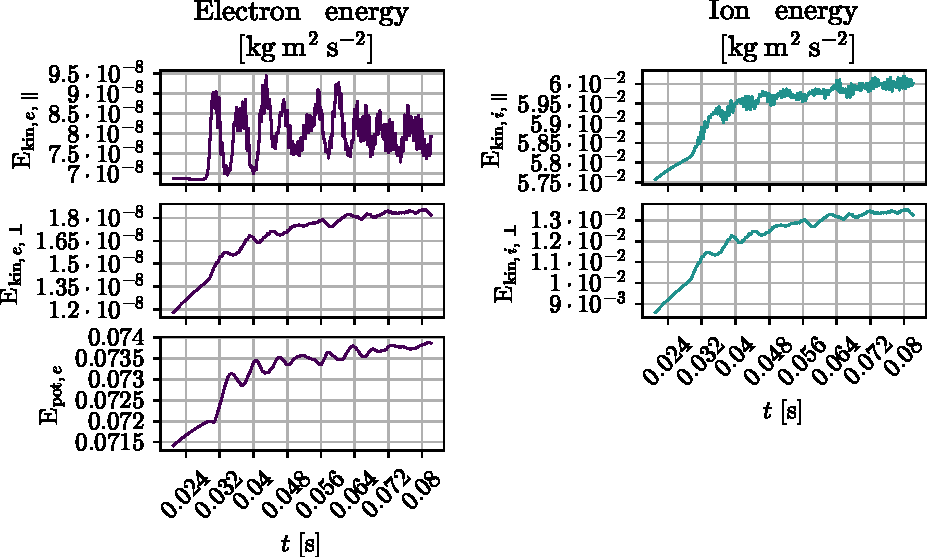
\includegraphics{fig/results/compareBouss/energies008B}
    \caption{Time trace of the energy for $B=0.08\T$ using the Boussinesq approximation.}
    \label{fig:energies008B}
\end{figure}
%
Firstly, in contrast to what is observed in simulations without the Boussinesq approximation, the energy is increasing in the linear phase (with exception of the parallel electron energy, which after close inspection actually shows a slight decrease in the linear phase).
For the potential energy, this means that the total number of particles in the system is increasing as the electron temperature and volume is constant.
If the density is increasing, this would also explain why the other energies are increasing as well.
The parallel electron energy can then only be decreasing if the parallel electron velocity is decreasing.

Next, the energy overshoot is absent for magnetic fields below $0.1\T$.
This fact can also be seen by visual inspection the temporal evolution of the fields.
The dynamics does not appear to be much faster during the onset of the turbulence then during the turbulent state.

Finally, the energy appears to be drifting to higher values with time.
In absolute terms, the energy is also larger when using the Boussinesq approximation.

This can also be seen if when investigating the temporal evolution of the fields.

Visual inspection of the fields also shows that the eddies evolves slower in the turbulence phase as when compared to the non-Boussinesq case.
Whereas the plasma in the CF develops filamentary structures, these structures are less pronounced in the CB case, and the plasma as a whole appear to be more coherent.
This can be seen by comparing \cref{fig:turbEv} with \cref{fig:turbBEv}
%
{
% FIXME: Move this figure and uncomment clearpage and thispage empty when document is done
% \clearpage
% \thispagestyle{empty}
\begin{figure}[htbp]
    \centering
    \begin{subfigure}[h]{1.00\textwidth}
        \centering
        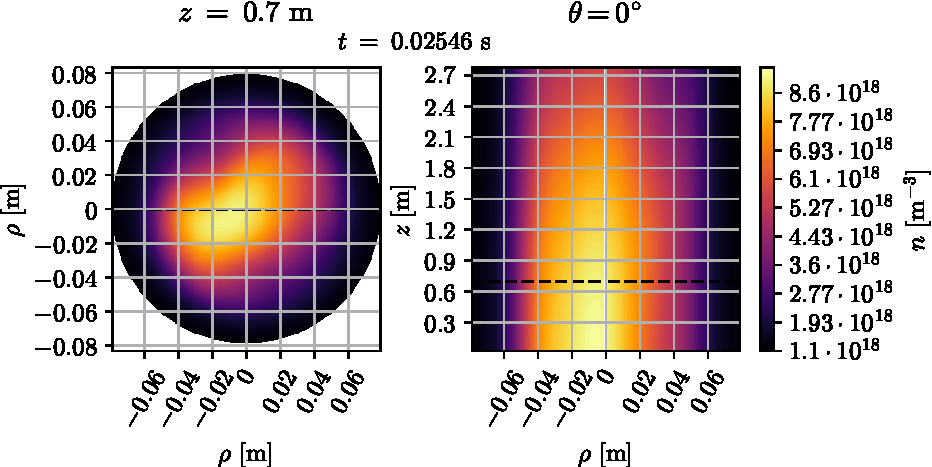
\includegraphics[width=1.0\textwidth]{fig/results/compareBouss/evolution/n-perpPar-2D-0}
    \end{subfigure}%
    \\
    \begin{subfigure}[h]{1.00\textwidth}
        \centering
        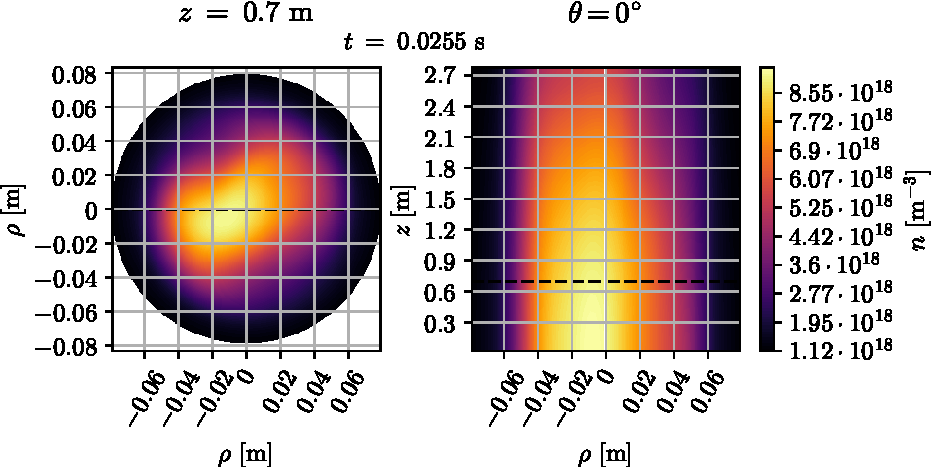
\includegraphics[width=1.0\textwidth]{fig/results/compareBouss/evolution/n-perpPar-2D-1}
    \end{subfigure}
    \\
    \begin{subfigure}[h]{1.00\textwidth}
        \centering
        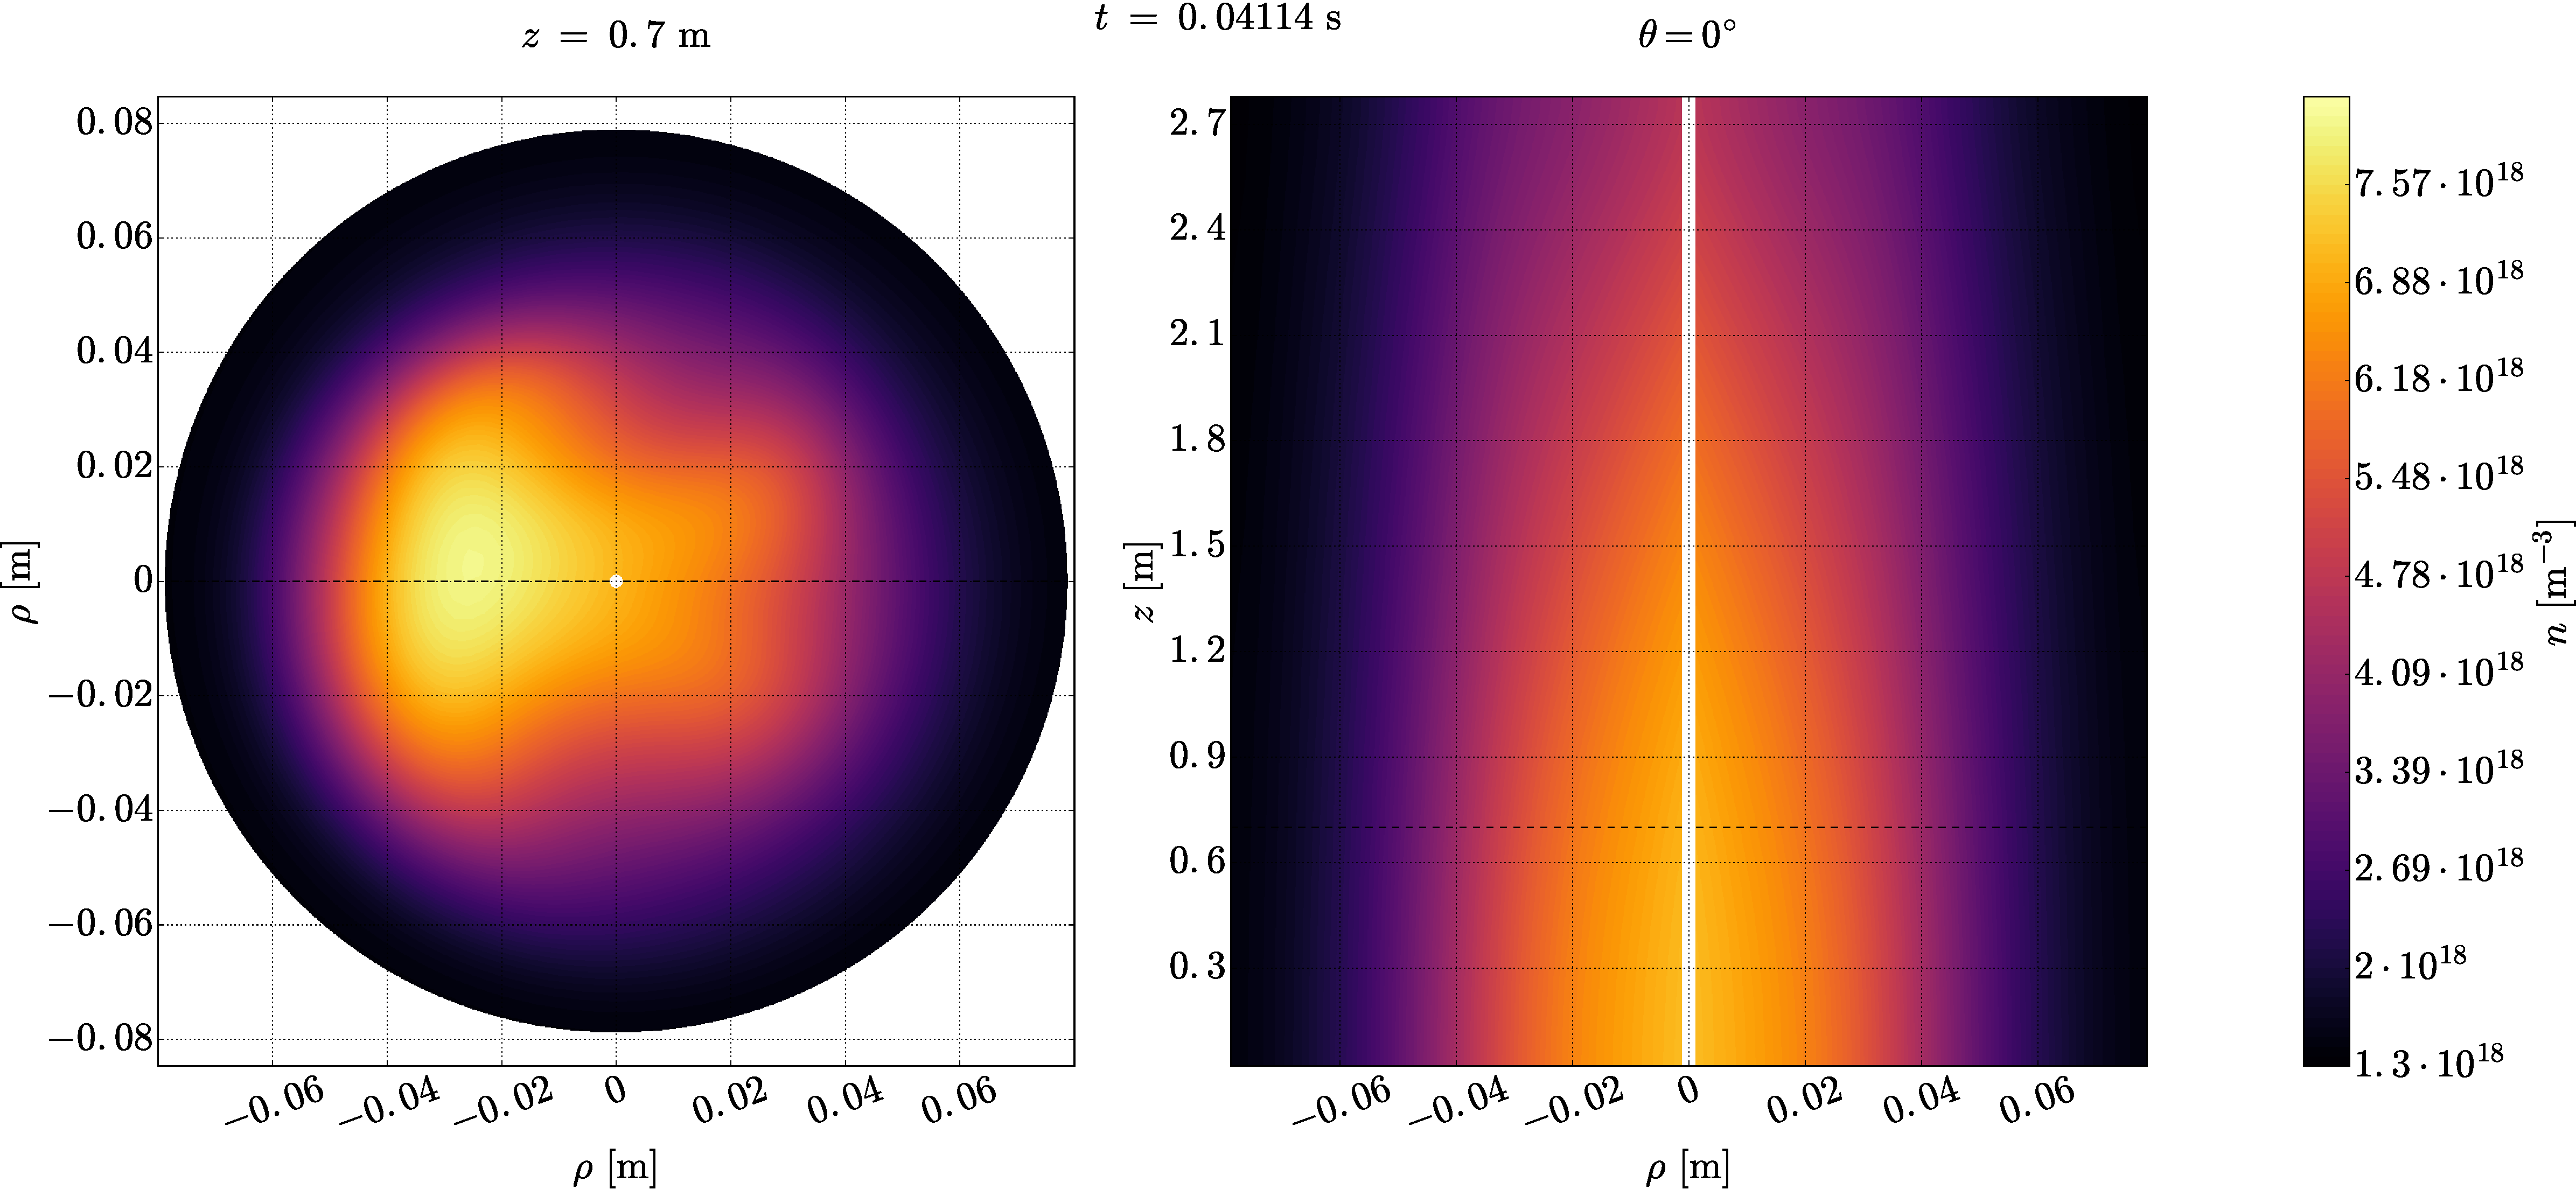
\includegraphics[width=1.0\textwidth]{fig/results/compareBouss/evolution/n-perpPar-2D-2}
    \end{subfigure}
    \caption{Evolution of the plasma in the saturated turbulence phase when using the Boussinesq approximation.
        Here shown for $B=0.08\T$}
    \label{fig:turbBEv}
\end{figure}
% \clearpage
}
%

\subsection{Fluxes}
%
Related to the drift in the energies as a function of time is the particle flux in the system.
This is depicted in \cref{fig:fluxB0008}.
%
\begin{figure}[htb]
    \centering
    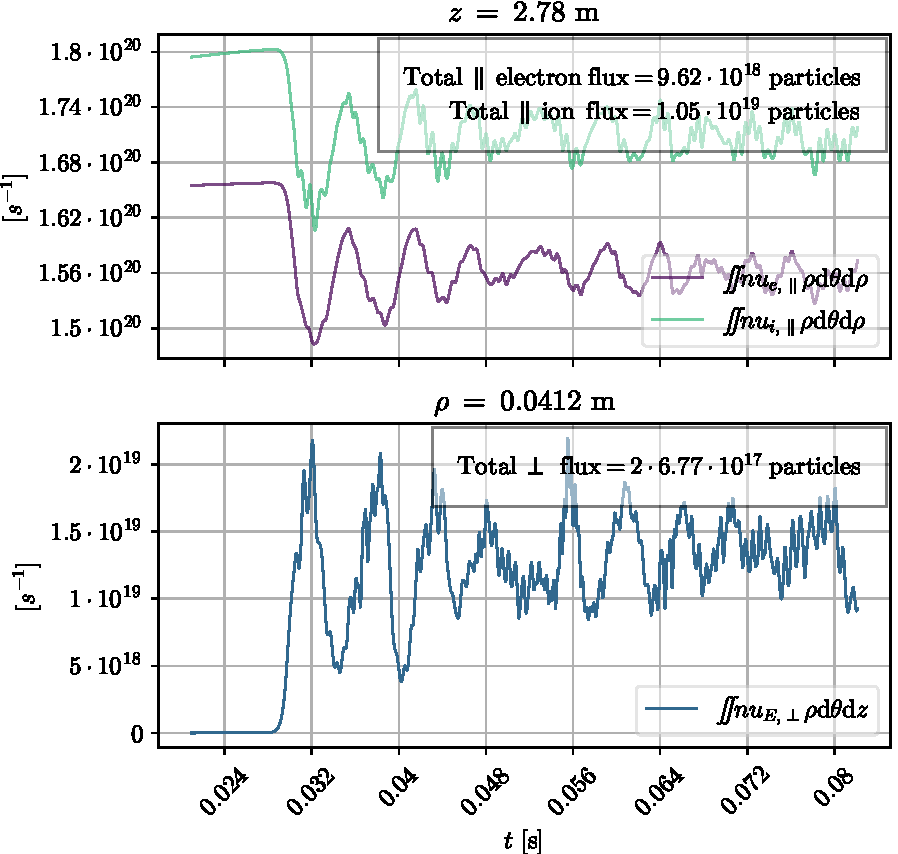
\includegraphics{fig/results/compareBouss/flux0008B}
    \caption{Integrated flux for $B=0.08\T$ using the Boussinesq approximation.}
    \label{fig:fluxB0008}
\end{figure}
%
It is apparent that there are more ions than electrons being lost in the system.
As a consequence, the plasma will be negatively charged with time.
Moreover, the continuous charging of the plasma will at some point break the quasi-neutral assumption, which is one of the back-bone assumptions in the drift-fluid approximation, and therefore also in the CELMA model.
In other words, the Boussinesq approximation in the current form is not consistent with its own assumptions.

Besides this very important fact, we can observe that the parallel fluxes in the CB case is of the same order of magnitude as the CF case, with the CB ion flux exceeding that of the CF case.
Furthermore, the perpendicular flux is less than half of what it is in the CF case.
This is consistent with the observation of less filamentation of the plasma as mentioned above.


\section{Fluctuations}
%
The rotation of the plasma structure is also apparent in the time traces of $n$ in the three positions around the maximum gradient.
This is shown in \cref{fig:comb008B}.
%
\begin{figure}[htb]
    \centering
    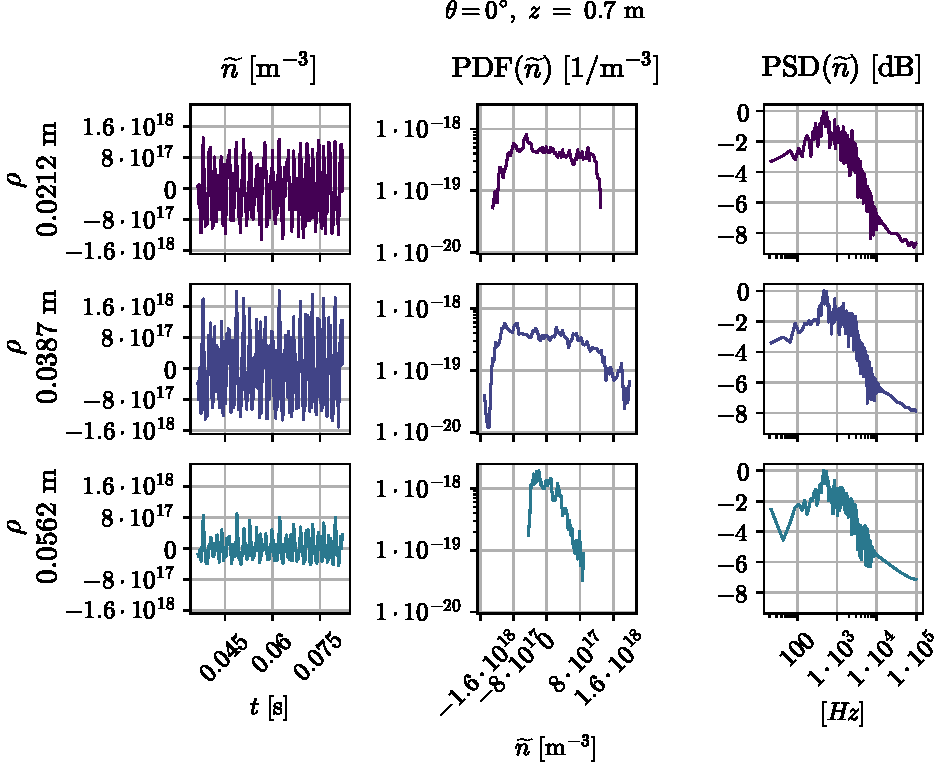
\includegraphics{fig/results/compareBouss/comb008B}
    \caption{Time traces in three fixed positions around the maximum gradient for $B=0.08\T$.}
    \label{fig:comb008B}
\end{figure}
%
First, we can not that the position of the maximum gradient is shifted slightly outwards.
Secondly, the time trace of the density fluctuation appears to be more ordered, in the sense that they appear more periodic than those observed in \cref{fig:combinedPlots008} for the CF case.
In the CB case the maximum of the power density spectrum is shifted to a higher frequency by a factor of approximately $3$, and falls off at a slightly faster rate than for the CF case.
Next, the PDFs are closer to Gaussian statistic as compared with the CF case.

This can also be seen from the skewness and excess kurtosis as a function of radial position, which is depicted in \cref{fig:skewKurt008B}.
%
\begin{figure}[htb]
    \centering
    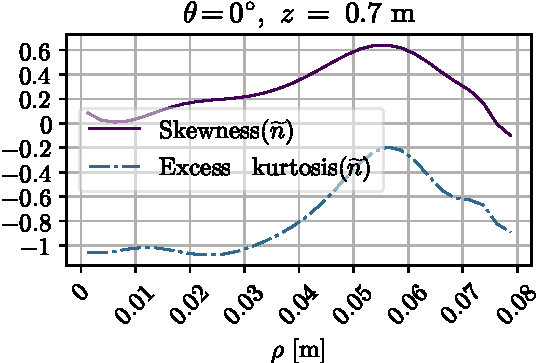
\includegraphics{fig/results/compareBouss/skewKurt008B}
    \caption{Skewness and kurtosis for $B=0.1\T$ using the Boussinesq approximation.}
    \label{fig:skewKurt008B}
\end{figure}
%
We observe that the system is platikurtic for all radii, meaning that there are less extreme events as compared with the non-Boussinesq case.
The skewness also less when using the Boussinesq approximation.
Both these facts reflects that the plasma is rotating around the center of the cylinder with a coherent character.

The lower fluctuation amplitude can also be seen in \cref{fig:fluctProfiles01B}, where one can observe that the profiles are less flattened than in the CF case.
Outside the position of the absolute maximum gradient the density profile follows the steady state profile to a good degree.
Furthermore, the potential is shifted closer to the absolute maximum of the gradient in the steady state.
%
\begin{figure}[htb]
    \centering
    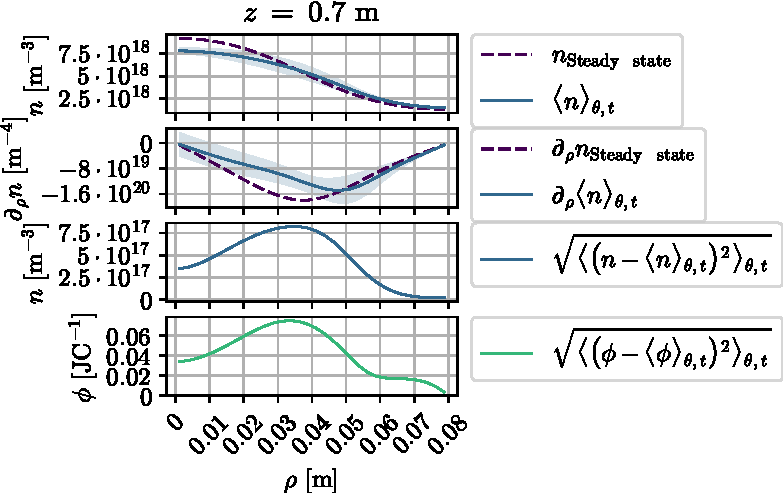
\includegraphics{fig/results/compareBouss/fluctProfiles01B}
    \caption{Steady state and averaged turbulent density profiles together with the radial distribution of the standard deviations of the fluctuations using the Boussinesq approximation with $B=0.1\T$.}
    \label{fig:fluctProfiles01B}
\end{figure}
%
